\section{System Architecture}
\begin{frame}
\frametitle{System Architecture}
What would this kind of overlay system look like?
\begin{itemize}
\item<2-> \textit{Meta-Model}
\item<3-> \textit{Non-Hierarchical Overlays}
\item<4-> \textit{Hierarchical Overlays}
\item<5-> \textit{Ontologies and Taxonomies}
\end{itemize}
\
\newline
\newline
\pause
\textit{...and what would the migration path to these systems look like?}
\end{frame}

\begin{frame}[t]
\frametitle{System Architecture - Level $\phi$}
\begin{figure}[!t]
\centering
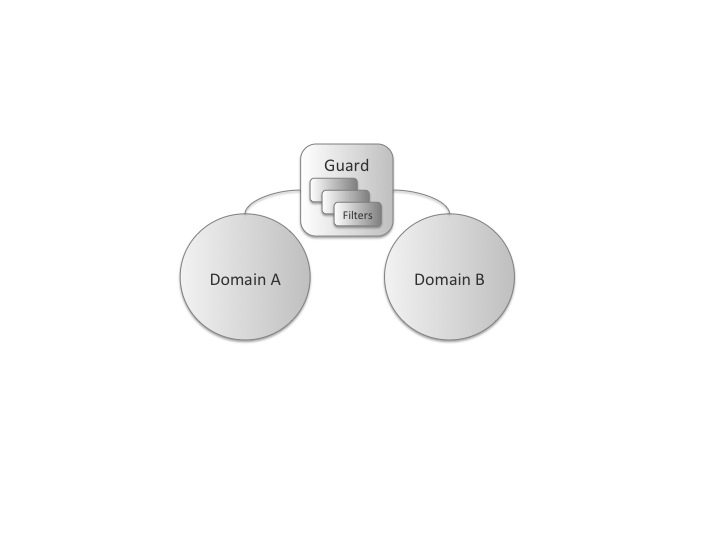
\includegraphics[width=3.4in]{model-phi}
\label{fig:model:phi}
\end{figure}
\end{frame}

\begin{frame}[t]
\frametitle{System Architecture - Level $\alpha$}
\begin{figure}[!t]
\centering
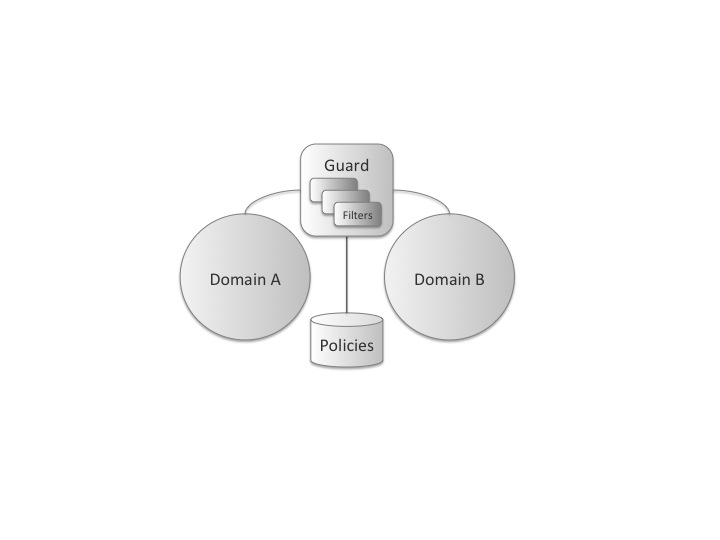
\includegraphics[width=3.4in]{model-alpha}
\label{fig:model:alpha}
\end{figure}
\end{frame}

\begin{frame}[t]
\frametitle{System Architecture - Level $\beta$}
\begin{figure}[!t]
\centering
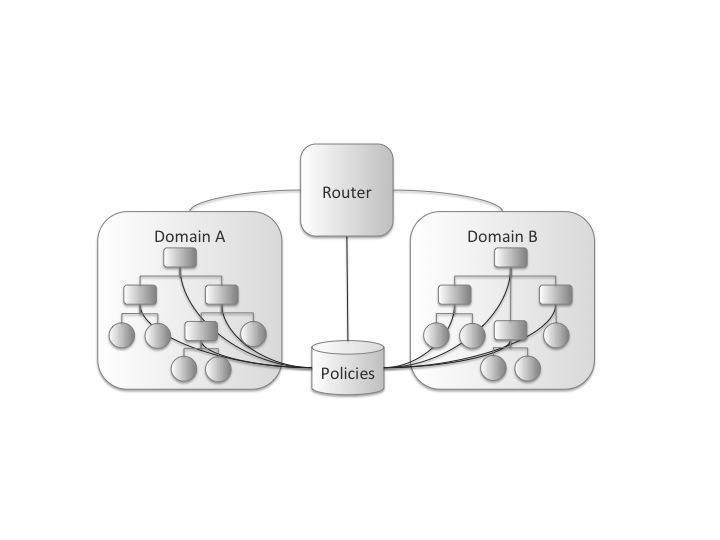
\includegraphics[width=3.4in]{model-beta}
\label{fig:model:beta}
\end{figure}
\end{frame}

\begin{frame}[t]
\frametitle{System Architecture - Level $\gamma$}
\begin{figure}[!t]
\centering
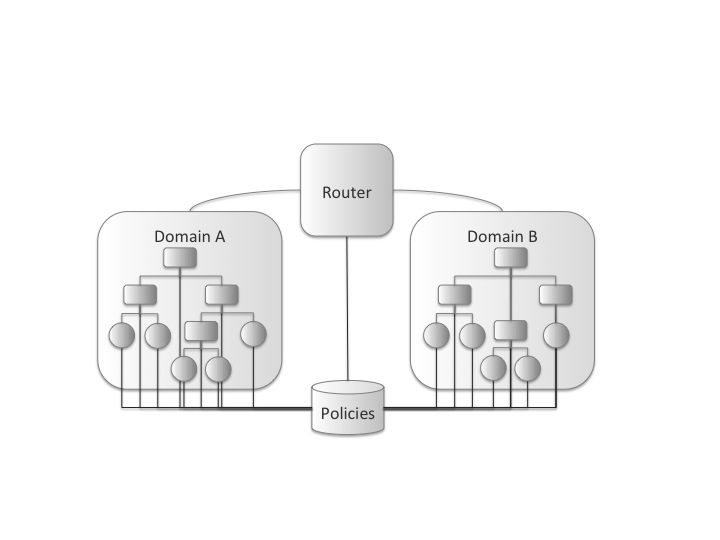
\includegraphics[width=3.4in]{model-gamma}
\label{fig:model:gamma}
\end{figure}
\end{frame}

\begin{frame}[t]
\frametitle{System Architecture - Level $\delta$}
\begin{columns}[t]
\column{.5\textwidth}
Level 3 system 
\column{.5\textwidth}
Fully Integrated Policy Aware Decentralized System
\end{columns}
\end{frame}